\documentclass[12pt]{article}
\usepackage{graphicx}

\title{Primer on Machine Learning and Deep Learning Techniques}
\author{Benjamin Li}
\date{2025}
\usepackage{setspace}
\usepackage{amsmath}
\usepackage{color,soul}
\usepackage{amsmath}
\usepackage{nicefrac}
\usepackage{amsfonts}
\usepackage{amsthm}
\usepackage{float}
\usepackage{csquotes}

\usepackage{hyperref}
\usepackage[margin=1in]{geometry}
\renewcommand{\baselinestretch}{1.5} 

\newcommand{\lnn}[1]{%
  \ln\left(#1\right)%
}

\newcommand{\logp}[1]{%
  \log\left(#1\right)%
}

\newcommand{\sigp}[1]{%
  \sigma\left(#1\right)%
}


\begin{document}
\interfootnotelinepenalty=10000

\maketitle
\tableofcontents
\newpage

\section{Introduction}

This document serves as an aggregation of my progress towards gaining a more fundamental understanding of how many modern ML/DL models work. I hope it can also serve as helpful pedagogical tool for those interested in learning about the inner workings of these algorithms (although some of it's more on the casual side and doesn't get into ALL the mathy details). This primer assumes basic knowledge in linear algebra, calculus, and probability. Corresponding code implementations will be made available in the future, and some helpful references for further learning are included for each section. 

This document is also a bit text-dense so I hope to increase the number of visuals (e.g. diagrams/drawings) with time. All figures are created by myself unless stated otherwise. I primarily use and highly recommend \href{draw.io}{draw.io} to create illustrations. 

\newpage
\section{Multilayer Perceptron (MLP)}
\begin{figure}[H]
    \centering
    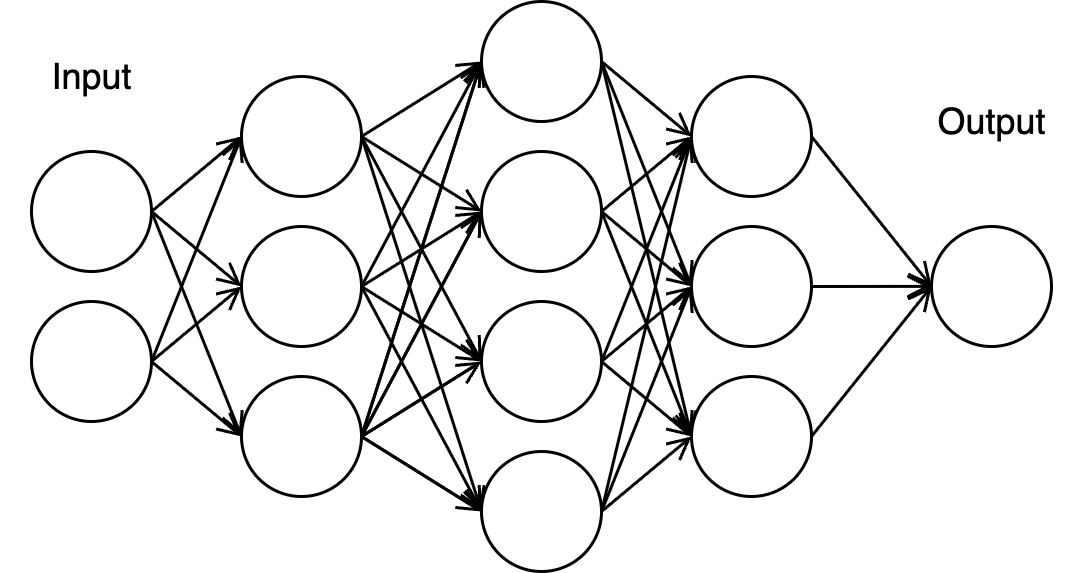
\includegraphics[width=0.8\textwidth]{../media/mlp.png}
    \caption{Multilayer Perceptron with three hidden layers.}
    \label{fig:mlp}
\end{figure}

A Multilayer Perceptron (MLP) AKA fully-connected neural network (FCN) is one of the most fundamental yet powerful algorithms in deep learning. At a high level, each of the \enquote{neurons} in the MLP represents some linear equation $y=mx+b$ with the output going through a nonlinear activation function $\sigma$. Applying a bunch of these operations in sequence enables us to model complex relationships without manually crafting a bunch of \enquote{if statements}. 

The key to creating and leveraging the network is linear algebra and calculus. Let's look at a specific example: we are given 10 soccer players and two pieces of info (\textbf{features}) about their goals per game and pass accuracy. We want to determine if they're going to be drafted to a soccer team. More formally, we are given a batched input $x$ of dimensions $(b, f)$, where $b$ is the number of entries and $f$ is the number of features - say $(10, 2)$. We are trying to predict a vector $y$ of dimensions $(10, 1)$ where 1 indicates that a player is drafted and 0 indicates they are not drafted. 

\[x=\begin{bmatrix}
50 & 75 \\
80 & 68 \\
100 & 80 \\
\vdots & \vdots \\
40 & 60
\end{bmatrix}, y=\begin{bmatrix}
0 \\
1 \\
1 \\
\vdots \\
0
\end{bmatrix}\]

To do this, we construct a neural network consisting of multiple \textbf{layers}, and within each layer multiple \textbf{neurons}. Then, initialize an array $n = [2, 3, 4, 3, 1]$ in which each index represents the number of neurons for the corresponding layer. Notably, the index 0 represents the INPUT dimension (number of initial features), and index 4 is the OUTPUT dimension (1 for 1 outcome). Finally, randomly initialize a list of weights and biases (more details later). Now, we have constructed the exact network described in Fig. \ref{fig:mlp}. The next step is training the network - updating its weights to more accurately model the training data. Training involves two steps: \textbf{feedforward} and \textbf{backpropagation}, covered in the subsequent two sections.  


\subsection{Feedforward Process}

Each layer $i$ calculates the following:
\[A_i = \sigma(W_i * A_{i-1} + B_i)\]

where $A_i$ is the \enquote{activated} output of the layer, $W_i$ is a weight matrix, $B_i$ is the bias matrix, and $\sigma$ is some activation function (e.g. sigmoid, relu) that introduces non-linearity. The intuition is that the weight matrices will automatically learn how to extract meaningful features from the data. However, we'll also need the \textbf{unactivated} output later for backpropagation: $Z_i = W_i * A_{i-1} + B_i$. We randomly initialize weight matrices with dimensions $(n_{i}, n_{i-1})$ and bias matrices of dimensions $(n_{i}, b)$. To understand why these dimensions are used, let's look at what happens after we pass through the \textbf{first} hidden layer of the network. We treat the original input X as the precursor activated value since there doesn't exist at this point. 

\[A_1 = \sigma(W_1 * X^T + B_1)\]

Note that we first transpose $X$, changing dimensions from (10, 2) $\rightarrow$ (2, 10). Then, left-multiply $X$ by $W_1$, yielding $(3,2) * (2,10) \rightarrow (3,10)$. Next, broadcast $B_1$ from $(3,1) \rightarrow (3,10)$ and add to the result. Pass the result into a nonlinear activation function $\sigma$, such as sigmoid or ReLU. For future iterations, use the previous activation value as input to calculate the value of Z. For instance, $Z_2 = W_2 * A_1 + B_2 \rightarrow (4, 3) * (3, 10) + (4, 10) \rightarrow (4, 10)$. Then, apply the activation function to find $A_2 = \sigma(Z_2)$, repeating for later layers until yielding $A_n=\hat{y}$. As mentioned earlier, it's a good idea to store all activated and unactivated values as they will be required during backpropagation. 

\subsection{Backpropagation}
Given some output $\hat{y}$, how can we tweak the weights and biases to more accurately predict the ground truth vector $y$? Mathematically, we try to minimize some loss/cost function $C$ with respect to weights and bias values. There are many choices available for $C$ that are good for different kinds of problems. One such loss function is called binary cross-entropy loss - it looks like this:

\[ C = -[y * \log{\hat{y}} + (1-y) * \log{(1-\hat{y})}] \]

Our goal is to calculate $\frac{dC}{dW_i}$ and $\frac{dC}{dB_i}$. This tells us how much cost is affected by the weights from that layer - once we know this information, we can move in the OPPOSITE direction of the gradient by some factor (learning rate, lr) to minimize the cost. In other words, we want to update the weights and bias this way: $W_i = W_i - lr * \frac{dC}{dW_i}$ and $B_i = B_i - lr * \frac{dC}{dB_i}$ (yes, this is programming notation). The first derivative to calculate is from the final weight matrix: $\frac{dC}{dW_3}$, found via the \textbf{chain rule}!

In our example, we need to get $\frac{dC}{dA_3}$ by taking the derivative of $C$ with respect to input. This turns out to be $-(\frac{Y}{\hat{y}} - \frac{(1-Y)}{1-\hat{y}})$, where $\hat{y}$ is equivalent to $A_3$. Then, $\frac{dA_3}{dZ_3}$ is just the derivative of the activation function, and $\frac{dZ_3}{dW_3}$ is the previous activation value at that index (because $Z_i = A_{i-1} * W_i + B_i$). This is represented by:

$$\frac{dC}{dW_3} = \frac{dC}{dA_3} * \frac{dA_3}{dZ_3} * \frac{dZ_3}{dW_3}$$ 

We will simplify this expression by assigning $\delta_3=dC/dZ_3$, so it becomes:

$$\frac{dC}{dW_3} = \delta_3 * \frac{dZ_3}{dW_3}$$

Next, to find $\frac{dC}{B_3}$, it is simply:

$$\frac{dC}{dB_3} = \delta_3 * \frac{dZ_3}{dB_3}$$

but conveniently $\frac{dZ_3}{dB_3} = 1$, so $\frac{dC}{dB_3} = \delta_3$!

Next, to find the derivatives of costs with respect to the other weights, we use the chain rule again! First, find the derivative of the cost vs. post-activation value for the next layer (layer 2 in our case). 

$$\frac{dC}{dW_2} = \delta_3 * \frac{dZ_3}{dA_2} * \frac{dA_2}{dZ_2} * \frac{dZ_2}{dW_2}$$

For the bias:
$$\frac{dC}{dB_2} = \delta_3 * \frac{dZ_3}{dA_2} * \frac{dA_2}{dZ_2} * \frac{dZ_2}{dB_2}$$

If we wanted to keep going, we would do the following. For the derivative of cost with respect to weight, omit the last operation ($\frac{dZ_2}{dW_2}$) and multiply $\frac{dZ_2}{dA_1} * \frac{dA_1}{dZ_1} * \frac{dZ_1}{dW_1}$. Similar idea with bias: omit $\frac{dZ_2}{dB_2}$ and replace with $\frac{dZ_2}{dA_1} * \frac{dA_1}{dZ_1} * \frac{dZ_1}{dB_1}$. For each layer, update the weights/biases using the new derivative values: $W_i = W_i - lr * \frac{dC}{dW_i}$ and $B_i = B_i - lr * \frac{dC}{dB_i}$. 

Ok, that was a lot... thankfully many libraries such as PyTorch have autodifferentiation features which can automatically perform the chain rule for us. \textbf{But it's important to know that not all loss functions are differentiable}! Also, although MLPs are universal function approximators with even a single hidden layer, it is unknown how many neurons are necessary for an arbitrary task. This is especially evident when trying to apply MLPs to image processing - and this motivates the next section on Convolutional Neural Networks (CNNs)! 


\subsection{Resources}
\begin{itemize}
  \item \href{https://www.nature.com/articles/323533a0}{Read the original backpropagation paper by Hinton and colleagues}
  \item \href{https://playground.tensorflow.org}{Interactive MLP simulation}
  \item \href{https://www.youtube.com/watch?v=IHZwWFHWa-w}{3B1B video on gradient descent, great for building strong visual intuition}
  \item \href{https://medium.com/@waadlingaadil/learn-to-build-a-neural-network-from-scratch-yes-really-cac4ca457efc}{Learn to Build a Neural Network from Scratch}
\end{itemize}

\newpage
\section{Convolutional Neural Networks}

Convolutional Neural Networks (CNNS) have been around for a while, but the first real breakthrough came when GPUs were discovered to greatly accelerate them. Then, the creation of AlexNet in 2012 kicked off its widespread usage in computer vision tasks. Now, there are many variants of CNNs used for many purposes ranging from image classification, object detection, segmentation, data compression, analyzing audio/time series data, image reconstruction, etc. To get a sense for how they work, we'll look at a \enquote{vanilla} CNN for classification (specifically for numbers, like the famous \href{https://en.wikipedia.org/wiki/MNIST_database}{MNIST} dataset), composed of two parts:

\begin{enumerate}
  \item Convolution layers
  \item Pooling layers
  \item MLP\footnote{Some CNNs are fully convolutional, but MLP is helpful for classification. }
\end{enumerate}

The convolution layers perform feature extraction, reducing the spatial size of the data in exchange for increased semantic depth. The MLP works the same as the aforementioned MLP, the only difference being that the input is a feature-dense representation of the original image data instead of being raw pixel values. The MLP's role is to output ten neurons, each indicating the network's \enquote{confidence} that the provided image represents the corresponding number from 0-9. 

\subsection{Convolutional Layers}
When we say CNNs reduce the spatial dimensions of the data in exchange for increased semantic depth, what exactly does that mean? Each convolution layer consists of many kernels, or filters, each of which is a matrix. Let's say we have a $5 \times 5$ grayscale matrix representing a \enquote{0} shape (values closer to 1 are more solid).  

\[
\begin{bmatrix}
0.2 & 0.8 & 0.9 & 0.8 & 0.2 \\
0.8 & 0.1 & 0.1 & 0.1 & 0.8 \\
0.9 & 0.1 & 0.2 & 0.1 & 0.9 \\
0.8 & 0.1 & 0.1 & 0.1 & 0.8 \\
0.2 & 0.8 & 0.9 & 0.8 & 0.2 \\
\end{bmatrix}
\]

Can you see this? The human eye and brain are very good at recognizing patterns - we can immediately see that the values close to 1 form a 0 shape. But how is a computer supposed to grasp that concept? The key is applying KERNELS. 

\begin{figure}[H]
    \centering
    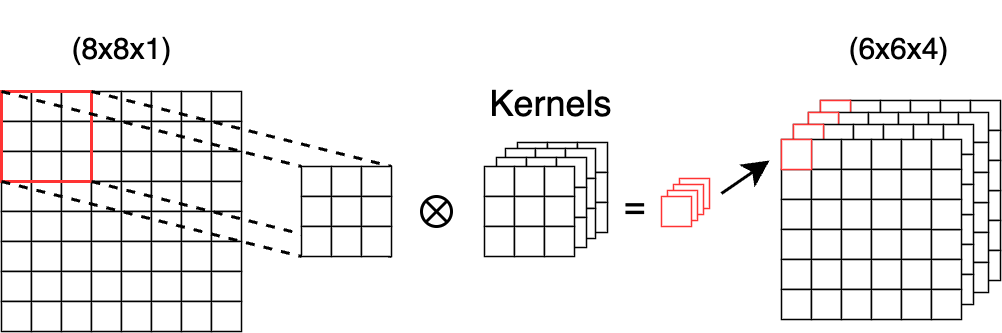
\includegraphics[width=0.8\textwidth]{../media/convolutions.png}
    \caption{Convolution operations visualized. }
    \label{fig:convolutions}
\end{figure}


As indicated in Fig. \ref{fig:convolutions}, these kernels are applied to data by taking the hadamard (element-wise) product of the original matrix with the filter followed by the sum. Then, the kernel "slides over" the entire image by a specified stride length, and the convolution operation is repeated until the entire input has been processed. Let's see if we can figure out what this kernel does:
\[
\begin{bmatrix}
1 & 1 & 1 \\
0 & 0 & 0 \\
-1 & -1 & -1 \\
\end{bmatrix}
\]

If we pass it over an image that's transitioning from dark to light (from top to bottom), the kernel will yield a very low value. This is because dark grayscale values are closer to zero than lighter grayscale values. Conversely, if it's going from light to dark, the kernel will yield a very high value. If it's the same color all the way through, the kernel will yield a value close to zero. This kernel captures \textbf{transitions into and out of horizontal edges}. 

This is the key: in exchange for reducing the dimensionality of a 3x3 patch to 1x1, we have extracted information about whether that region represents an edge. Because we have many different kernels, we can extract many types of features otherwise impossible for the machine to discern. As for how these kernels are found - they are actually randomly initialized and learned via backpropagation. 

\subsection{Pooling Layers}

Pooling operations (e.g. maxpool) are often used in tandem with convlayers. As with many things in deep learning, nobody knows exactly why pooling works so well but experimentally it's quite robust. Some theorize that it adds translational invariance (e.g. the max value within a window remains the same even if the features shift slightly) or is a mechanism for regularization.

The idea with pooling is very similar to conv layers - reducing the spatial dimensions of the data. However, something like maxpool actually loses information - selecting the maximum pixel value to represent an entire sliding window. In many cases, this can actually be beneficial if it discards noisy activations in favor of stronger signals. Also, it is preconfigured (i.e. doesn't require any parameters), improving efficiency over using all convolutional operations.
\begin{figure}[H]
    \centering
    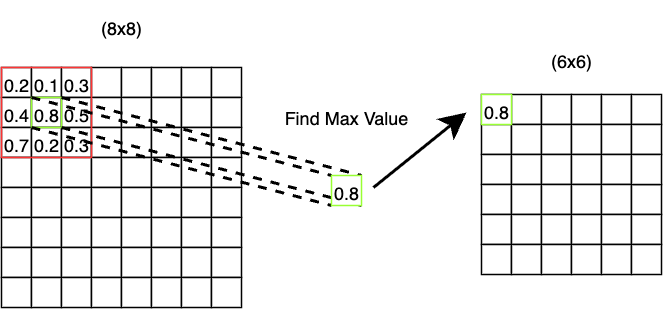
\includegraphics[width=0.8\textwidth]{../media/pooling.png}
    \caption{Max pool operation visualized. }
    \label{fig:pooling}
\end{figure}

\subsection{Resources}
\begin{itemize}
  \item \href{https://towardsdatascience.com/convolutional-neural-networks-explained-9cc5188c4939/}{CNN explained}  
  \item \href{https://poloclub.github.io/cnn-explainer/}{CNN explainer (hands-on)}
  \item \href{https://adamharley.com/nn_vis/cnn/3d.html}{Another cool CNN visualizer}
\end{itemize}

\newpage
\section{Transformers}

\begin{figure}[H]
    \centering
    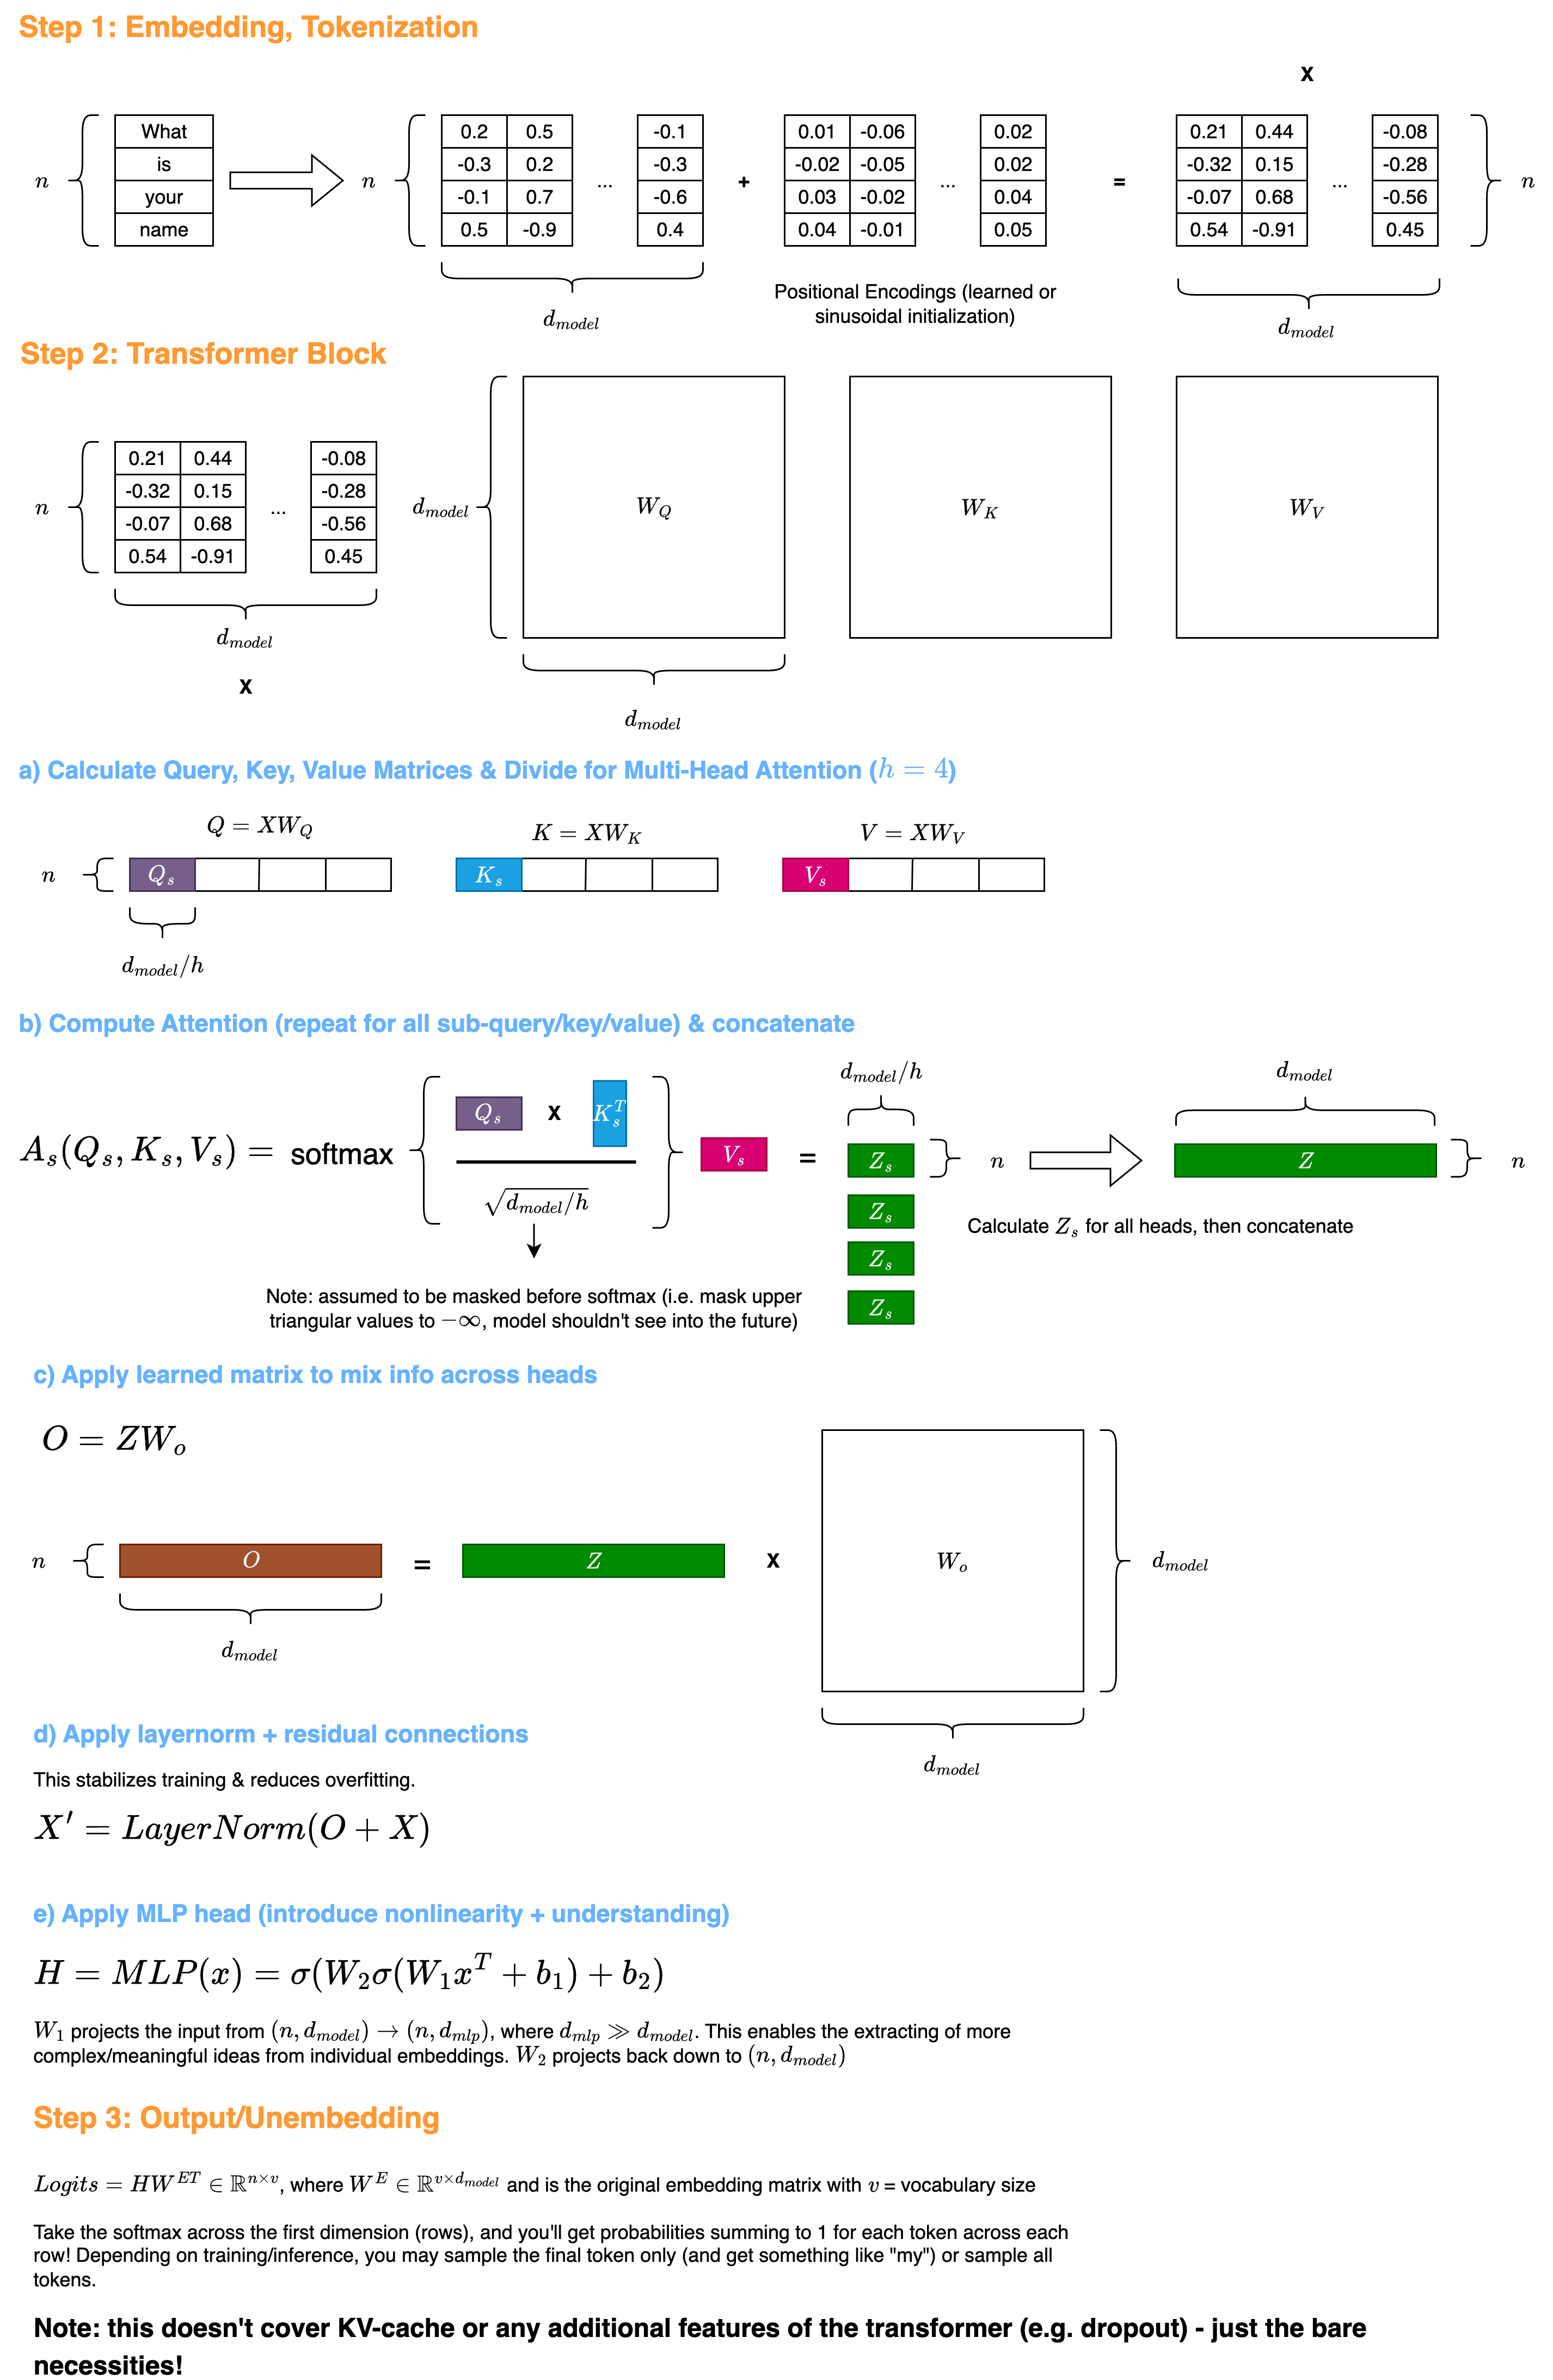
\includegraphics[width=0.8\textwidth]{../media/transformer.png}
    \caption{Transformer overview, individual parts discussed below. Zoom to read better!}
    \label{fig:transformer}
\end{figure}

Transformers are typically composed of three parts:
\begin{enumerate}
  \item \textbf{Embedding}: take some sentence composed of n words and embed those words using some algorithm into a higher dimensional space (n x $d_{model}$). Say that the model has a vocabulary size of $v$. This embedding algorithm basically maps a token within that vocabulary to $v \in \mathbb{R}^{d_{model}}$.
  \item \textbf{Transformer Blocks} (Multi-Head Attention + MLP): \enquote{reweight} each of the $n$ embeddings based on information from other embeddings. 
  \item \textbf{Output}: the \enquote{reweighted} embeddings get \enquote{unembedded}. The goal is to get a probability distribution over all possible tokens in the vocabulary for the next token after the current embedding.
\end{enumerate}


\subsection{Embedding}\label{sec: embedding}
\begin{figure}[H]
    \centering
    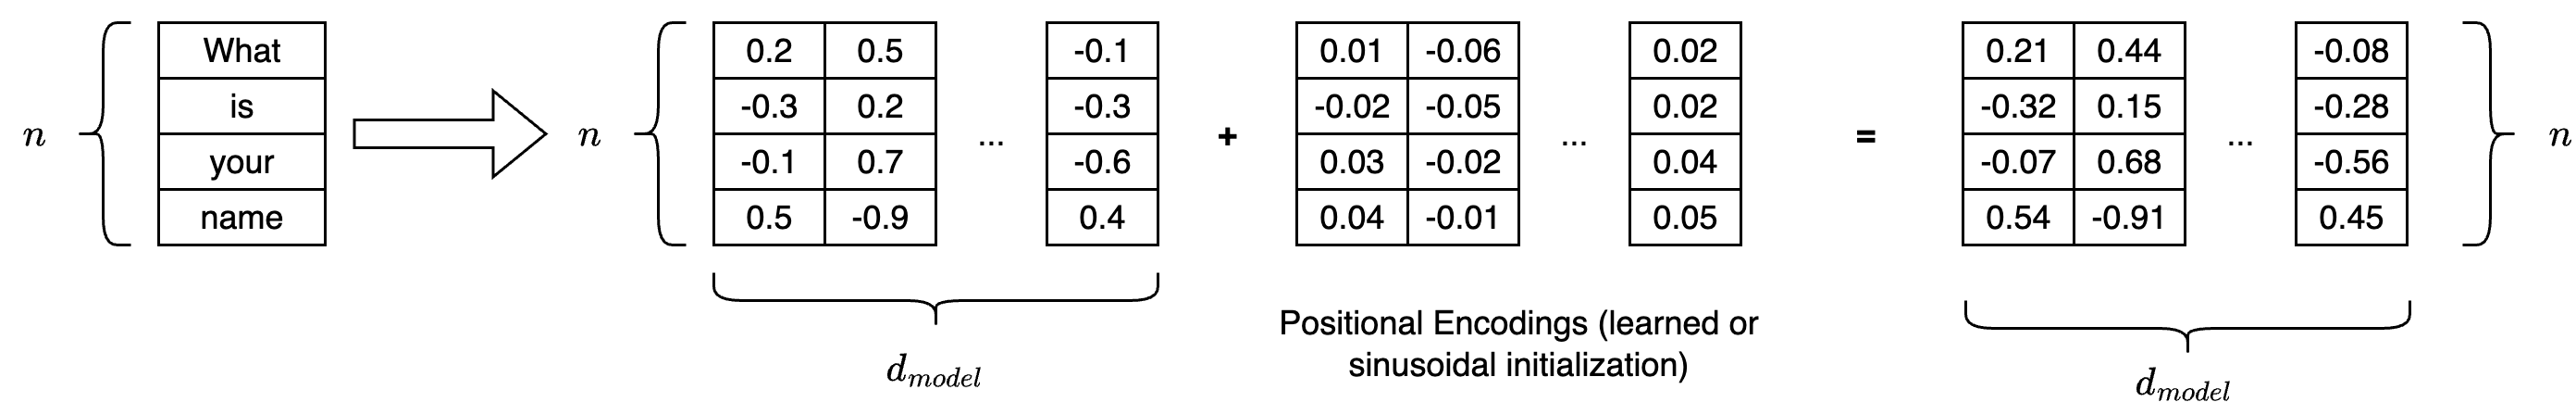
\includegraphics[width=0.8\textwidth]{../media/embedding.png}
    \caption{Embedding overview. }
    \label{fig:embedding}
\end{figure}

Given some sentence, such as \enquote{What is your name}, we first convert the sentence into tokens (i.e. vectors) such that each word maps to a unique token - a process called tokenization. For the English language, tokenization can be understood relatively simply as selecting each word and converting it into a vector representation. Notably, however, tokenization is still an open problem. Not all languages are tokenized equally - 
Burmese or Amharic may take up to 10x tokens to represent an equivalent message in English, as described in \href{https://medium.com/data-science/all-languages-are-not-created-tokenized-equal-cd87694a97c1}{this post}. This may lead to biased model performance for languages with patterns similar to English. 

As illustrated in the diagram above, let's say we have an array of words of length 4: [\enquote{What}, \enquote{is}, \enquote{your}, \enquote{name}], which for simplicity has been cleaned from punctuation and extraneous characters\footnote{What is \enquote{filtered out} depends on the specific tokenization strategy.}. For the purposes of conciseness, the batch size is assumed to be 1 but calculations can be simply made valid by broadcasting matrices to match dimensions. For example: instead of $(4 \times 512) * (512 \times 512) \rightarrow (4 \times 512)$, for batch size 3 we broadcast $(512 \times 512) \rightarrow (3 \times 512 \times 512)$. Thus, we get $(3 \times 4 \times 512) * (3 \times 512 \times 512) \rightarrow (3 \times 4 \times 512)$.

We want to convert each word in the array to $v \in \mathbb{R}^{d_{model}}$, where $d_{model}$ is the model depth and is $512$ in \enquote{Attention is All You Need} - the original transformer paper. Intuitively, it can be understood as how many concepts the model is able to compare between different tokens. The classical example is to take the embeddings of some words and perform operations such as $king-man+woman\approx queen$. A single index within a 512-D embedding doesn't mean much, but it does when taken together with everything else. Because these representations are so abstract, we still don't have a reliable way of mapping embeddings to concepts and vice versa\footnote{For more info, I recommend looking into the field of mechanistic interpretability starting with Anthropic's paper \href{https://transformer-circuits.pub/2023/monosemantic-features}{towards monosemanticity} - some really interesting stuff}. Positional encoding is then added to each vector word embedding, producing vectors of the same dimensions but allowing the model to understand the position of tokens relative to each other. With our four-word example, we obtain a $4 \times 512$ matrix as final output and refer to this as $X$. The positional encoding encoding can be deterministic via sinusoidal initialization (as in the original \enquote{Attention is All You Need} paper) or learned, as in some future papers. 

\subsection{Transformer Block}

The goal of the transformer block is to mix meaningful information across embeddings and sharpen their in-context meaning. There are two parts of each transformer block: multi-head attention and MLP layer. 

\subsubsection{Attention}

Before understanding multi-head attention, it's helpful to grasp \enquote{self-attention}. The goal of both types of attention is to generate a refined representation of our embeddings such that they incorporate relevant information from embeddings around them. 

\textbf{Self-attention}: we begin by creating three learnable weight matrices: $W_Q$, $W_K$, $W_V$, each dimensions $d_{model}$ for query, key, value respectively. Then, right-multiply $X$ by each of these matrices, creating three resulting matrices of the same dimensions $Q$, $K$, $V$. To understand what these matrices represent, I found it helpful to frame matrix multiplication as the dot product between every row in $X$ (i.e. token) and every column in $W$. Recall that the dot product between two vectors encodes similarity (i.e. high value = similar, low value = dissimilar). With this in mind, let's look at the query matrix $W_q$. Think of each column of $W_q$ as encoding some \enquote{search term}. Select an arbitrary row in the matrix $X$, say the first row. 

\[x_1 = \begin{bmatrix}
0.21 & 0.44 & ... & -0.08
\end{bmatrix}\]

Computing the dot products between that row and the columns of $W_q$ give you a vector with each element representing whether the current token is searching for a particular query. Repeat this logic for the key matrix, except this time instead of each column representing a \enquote{search} term it represents some abstract concept (hence \enquote{key}). Finally, find the value matrix $V$, representing information that's actually mixed. The dimensions of $Q$, $K$, $V$ are all $(n \times d_{model})$, $(4 \times 512)$ in our case.

Now that we have these matrices that are supposed to encode information from these tokens, we calculate the \textbf{attention} matrix. We first take the matrix product between $Q$ and $K^T$ - now each entry in the product represents how well a certain token's query aligns with another token's value. Then, divide by $\sqrt{d_{model}}$. Next, mask the upper triangle of the product (i.e. where $j > i$) to $-\infty$. Because of the autoregressive nature of the transformer, it should not be able to use future words to inform its prediction for the current word. Finally, take the softmax of the product such that all entries along a row/column sum to one. This gives us the \textbf{attention matrix} $A$ with shape $n \times n$ and $4 \times 4$ in our case. 

This is where the $V$ comes in. We left-multiply $V$ by $A$ to get $O$, the final output of the attention layer. Recall that each row $i$ of A represents the relevance of token $i$ to token $j \forall j<n$. Therefore, by doing this matrix multiplication, each element in a row of $O$ represents how much of token $j$'s value to include $i$'s new token representation. Thus, the final output of an attention layer can be understood as:

\[O = Attention(Q, K, V) = softmax(\frac{Q*K^T}{\sqrt{d_{model}}})V\]

Notably, after all these operations, $O \in \mathbb{R}^{n \times d_{model}}$ retains the same dimensions as the original input $X$, showing how what we did was essentially information across different tokens, up and down-weighting certain embeddings based on their relationships. 

\textbf{Multi-head attention}: in practice, having one giant matrix for each of $Q, K, V$ may \enquote{drown out} niche relationships - like a jack of all trades, master of none. This motivates the creation of multiple diverse, specialized attention \enquote{heads}, each of which focuses on a different aspect of language. What this entails is first subdividing the input X into $h$ heads and individually computing query, key, value matrices ($Q_i, K_i, V_i \in \mathbb{R}^{n \times d_{k}} \forall i \in h$), where $d_k=d_{model}/h$. Then we calculate \[A_i(Q_i, K_i, V_i)= softmax(\frac{Q_i*K_i^T}{\sqrt{d_k}})V_i, \forall i \in h\]

Each $A_i \in \mathbb{R}^{n \times d_{k}}$ is concatenated along the second (channel) dimension, producing $Z \in \mathbb{R}^{n \times d_{model}}$. We're not done yet - now that the heads have been concatenated, mixing information across heads could yield valuable results too. We therefore apply a learned matrix $W_O$ which right-multiplies $Z$ to yield $O = ZW_O, O \in \mathbb{R}^{n \times d_{model}}$. 

The last step in the transformer block is to apply \textbf{layer normalization} and \textbf{skip connections}. Layer normalization stabilizes training by calculating the standard deviation $\sigma_i$ and mean $\mu_i$ of all the features within each sample in the batch and doing z-score normalization with those statistics \footnote{Recall that in this demo, the batch size was 1 but reasoning can be simply extended to larger batch sizes. See section \ref{sec: embedding} for more info and an example.}. Skip connections allows us to avoid exploding/vanishing gradients. Thus, we compute our final output via $X' = LayerNorm(O + X)$. 

\begin{figure}[H]
    \centering
    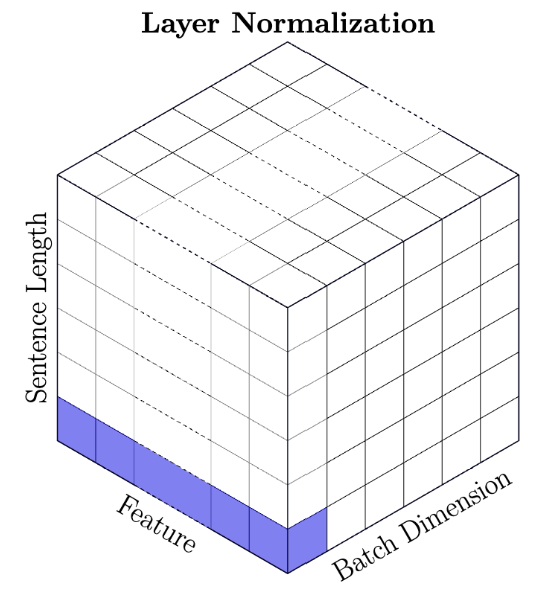
\includegraphics[width=0.5\textwidth]{../media/layernorm.png}
    \caption{Layer Norm visualization. \href{https://proceedings.mlr.press/v119/shen20e/shen20e.pdf}{Credit for this illustration}}
    \label{fig:norms}
\end{figure}



\subsubsection{MLP Layer}

% In our case, there are $d_{model}$ "search terms", but in theory this value could be different. 

Given the output from the transformer block $X' \in \mathbb{R}^{n \times d_{model}}$, we pass it into the multilayer perceptron (MLP) to introduce nonlinearity (not present in attention computations otherwise) and capture higher level facts about the input data. The MLP processes each token separately from the others with the following formula: 

$$H = MLP(x) = W_2\sigma(W_1X + b_1) + b_2$$

The important idea here is \(W_1\) projects the input from \((n, d_{model}) \rightarrow (n, d_{mlp})\),
where \(d_{mlp} \gg d_{model}\). The reason for selecting \(d_{mlp} \gg d_{model}\) is because projecting to a much larger dimensional space allows extraction of richer features. \(W_2\) projects the output back down to our original dimensions \((n, d_{model})\), yielding $H$. Oftentimes layernorm is also applied after the MLP. 

\subsection{Output}

Given some input $H$, the goal is to get 
\(Logits = HW^{ET}, Logits \in \mathbb{R}^{n \times v}, W^E \in \mathbb{R}^{v \times d_{model}}\). In English, take the transpose of the original embedding matrix $W^E$ and right-multiply $H$. A row of the resulting product represents the raw logits for every word in the model's vocabulary. Next, take the softmax across the vocabulary dimension (i.e. columns) - this makes logits for each word in the sentence sum to 1! 

Here is where the training/inference procedure differs. If it's training, calculate the cross-entropy loss between the ground truth next token and the predicted token for EVERY word in the sentence, backpropagating the loss to update all the weight matrices. If it's inference, just extract the most probable next token from the LAST word in the sentence. 

Notably, some transformer models have encoders AND decoders, whereas others are only encoders (e.g. BERT) and others are only decoders (e.g. GPT). They differ in use cases, namely that encoder-based models are good for capturing deep semantic information whereas decoder-based models can generate new, realistic output. However, the difference between encoder-only and decoder-only models has been blurring a bit as models from both sides improve their understanding and generation capabilities. Finally, it's important to know that transformers are useful outside natural language processing too. Vision transformers, which treat images as patches and linearly project those patches to a flattened embedding to feed into the model, have exploded in popularity recently. This is due to their superior ability to capture long-range dependencies vs. CNNs, but they occasionally struggle at low dataset size. Definitely suggest reading about them (link in the resources section). 


\subsection{Resources}
\begin{itemize}
  \item \href{https://arxiv.org/pdf/1706.03762}{Attention Is All You Need (Transformer paper)}
  
  \item \href{https://arxiv.org/abs/2010.11929}{Vision transformer paper}

  \item \href{https://github.com/hyunwoongko/transformer}{PyTorch transformer implementation}
  
  \item \href{https://www.youtube.com/watch?v=wjZofJX0v4M}{3B1B high-level overview of transformers}
  
  \item \href{https://www.youtube.com/watch?v=eMlx5fFNoYc}{3B1B video on attention - it's so good that I had to include two 3B1B videos}
  
\end{itemize}

\section{Training Models}

\subsection{LMs: Reinforcement Learning with Human Feedback (RLHF)}

\begin{figure}[H]
    \centering
    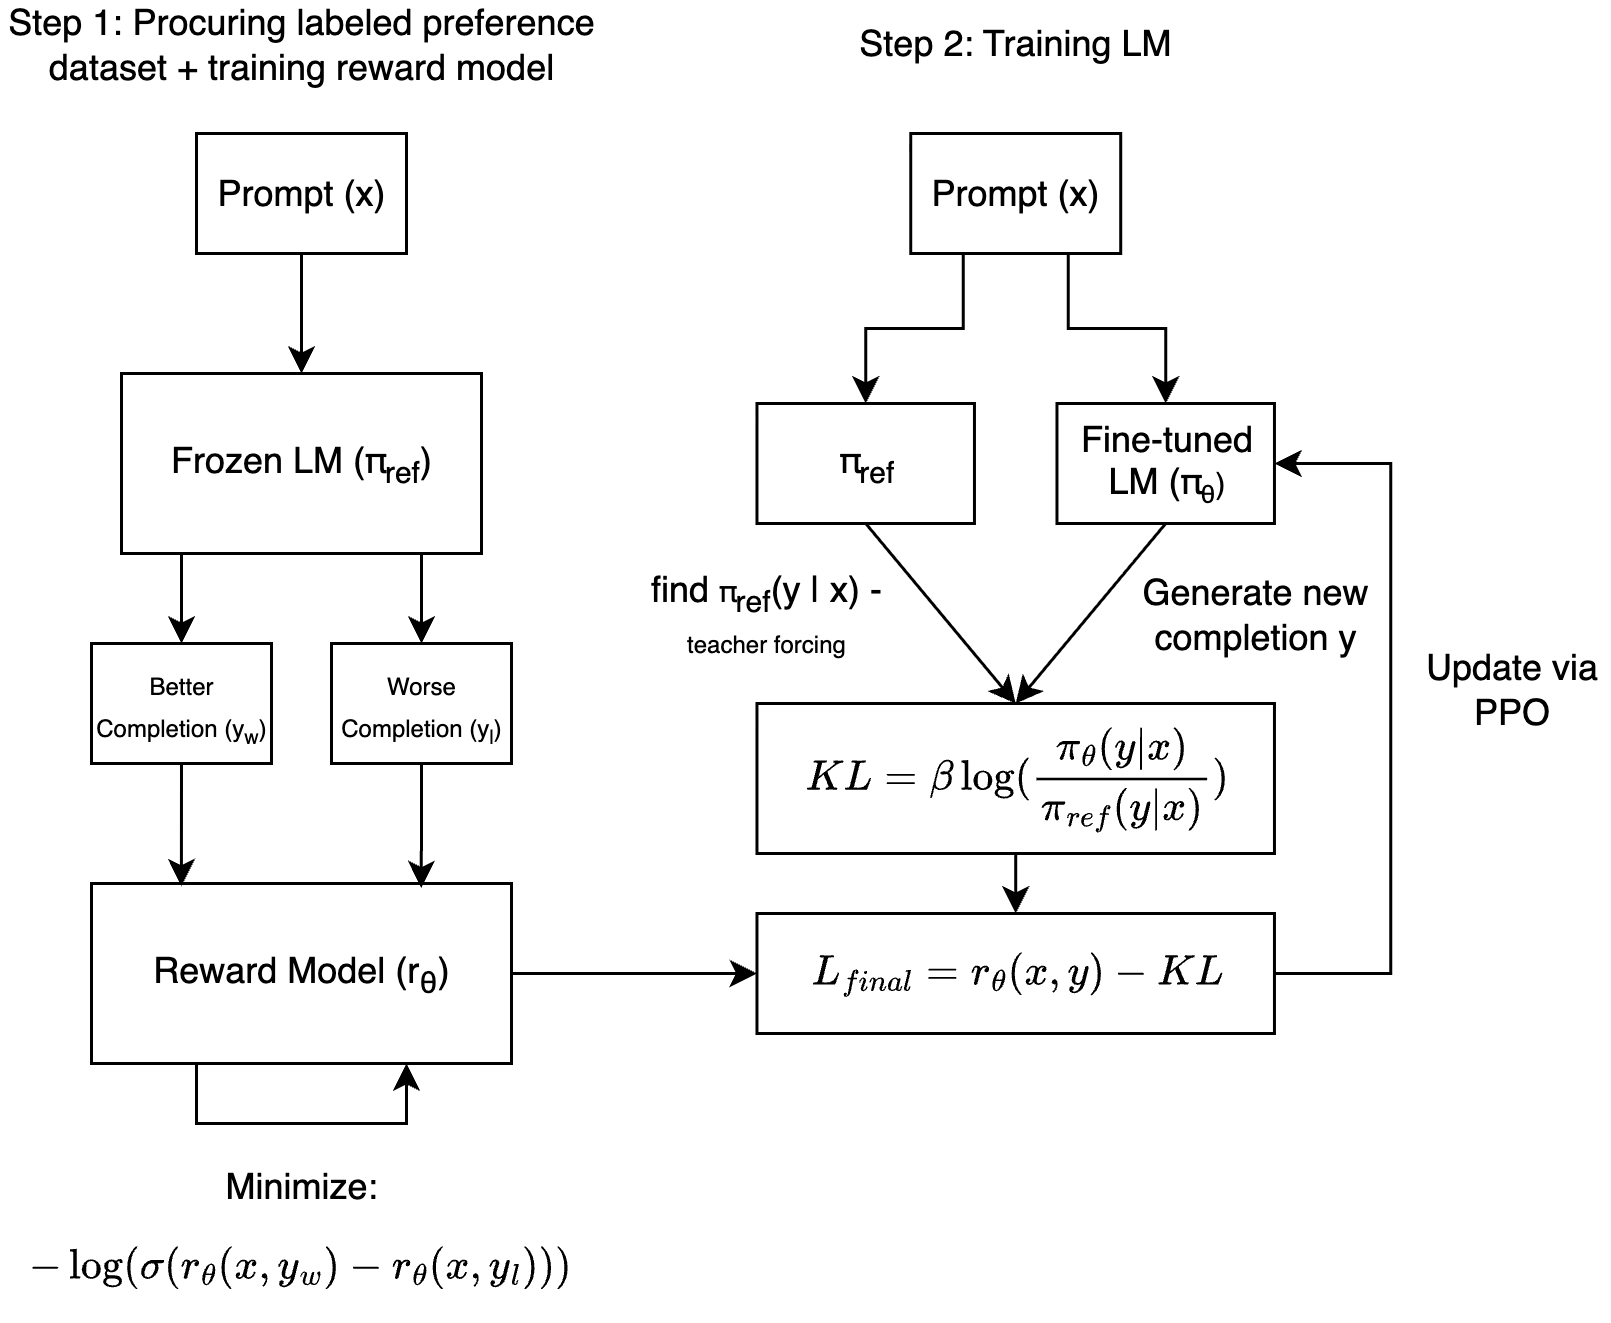
\includegraphics[width=1\textwidth]{../media/rlhf_light.png}
    \caption{RLHF overview. }
    \label{fig:rlhf}
\end{figure}

Given some language model (LM) that's been pretrained on a large corpus of data (e.g. internet), we don't know how \textbf{reliable} or \textbf{aligned} that data is with human values. Thus, we want to \textbf{guide} the LM to incorporate basic human values, such as honesty, harmlessness, etc. Here's a high level overview of the process:

\begin{enumerate}
    \item \textbf{Reward Model}: procure a dataset of good/bad LM outputs relative to a prompt (via human annotators), train a reward model to maximize the difference in reward between good/bad prompt. Freeze the reward model after training. 
    \item \textbf{KL Divergence Calculation}: for any given prompt, calculate the KL divergence between frozen and unfrozen version of LM and subtract from the reward model output. 
    \item \textbf{PPO gradient update}: update weights of the unfrozen LM, and repeat step 2 and 3 until satisfactory performance is achieved. 
\end{enumerate}

\subsubsection{Reward Model}
We want to first train a reward model that models human preference. Given a pretrained reference model $\pi_{\mathrm{ref}}$, for each prompt $x^{(i)}$ where $i = 1, \ldots, N$, generate two outputs $y_w^{(i)}$ and $y_l^{(i)}$ such that:
\[
y_w^{(i)}, y_l^{(i)} \sim \pi_{\mathrm{ref}}(\cdot \mid x^{(i)})
\]
where $y_w^{(i)}$ is the preferred (higher-quality) completion and $y_l^{(i)}$ is the less preferred (lower-quality) completion for prompt $x^{(i)}$. This yields a dataset of $(y_w^{(i)}, y_l^{(i)}, x^{(i)})_{i=1}^{N}$. 

Next, use a reward model $r_{\phi}$ (perhaps just a transformer an added linear layer at the end) to process each sample in the dataset, minimizing the loss 

\[L_{reward} = -\logp{\sigp{r_{\phi}(y_w) - r_{\phi}(y_l)}}\]. This encourages the maximization of the reward for the good response while minimizing the reward for the bad response. 

\subsubsection{KL Divergence Calculation + PPO update}
Now, we have a trained reward model. Let's freeze the weights of the original LM ($\pi_{ref}$) make a trainable copy of the original LM and call it $\pi_{\phi}$ (this will be the final fine-tuned LM after the entire process is complete). 

We need to prevent $\pi_{\phi}$ from \enquote{reward hacking} (i.e. giving nonsensical outputs to fool the reward model), so we calculate KL divergence between outputs of $\pi_{\phi}$ and $\pi_{ref}$. This is given as $KL = \beta\logp{\frac{\pi_{\phi}(y|x)}{\pi_{ref}(y|x)}}$. The further $\pi_{\phi}(y|x)$ is from $\pi_{ref}(y|x)$, the greater the KL divergence. 

To update the new LM $\pi_{\phi}$, calculate 

$$L_{final} = r_{\theta}(x,y) - KL$$

and use the proximal policy optimization (PPO) algorithm to backpropagate the loss. Broadly, PPO clips policy updates and restrains major updates to the model with the same motivation as KL divergence (read more about it in the link in references). 

\subsection{LMs: Direct Preference Optimization (DPO)}
\begin{figure}[H]
    \centering
    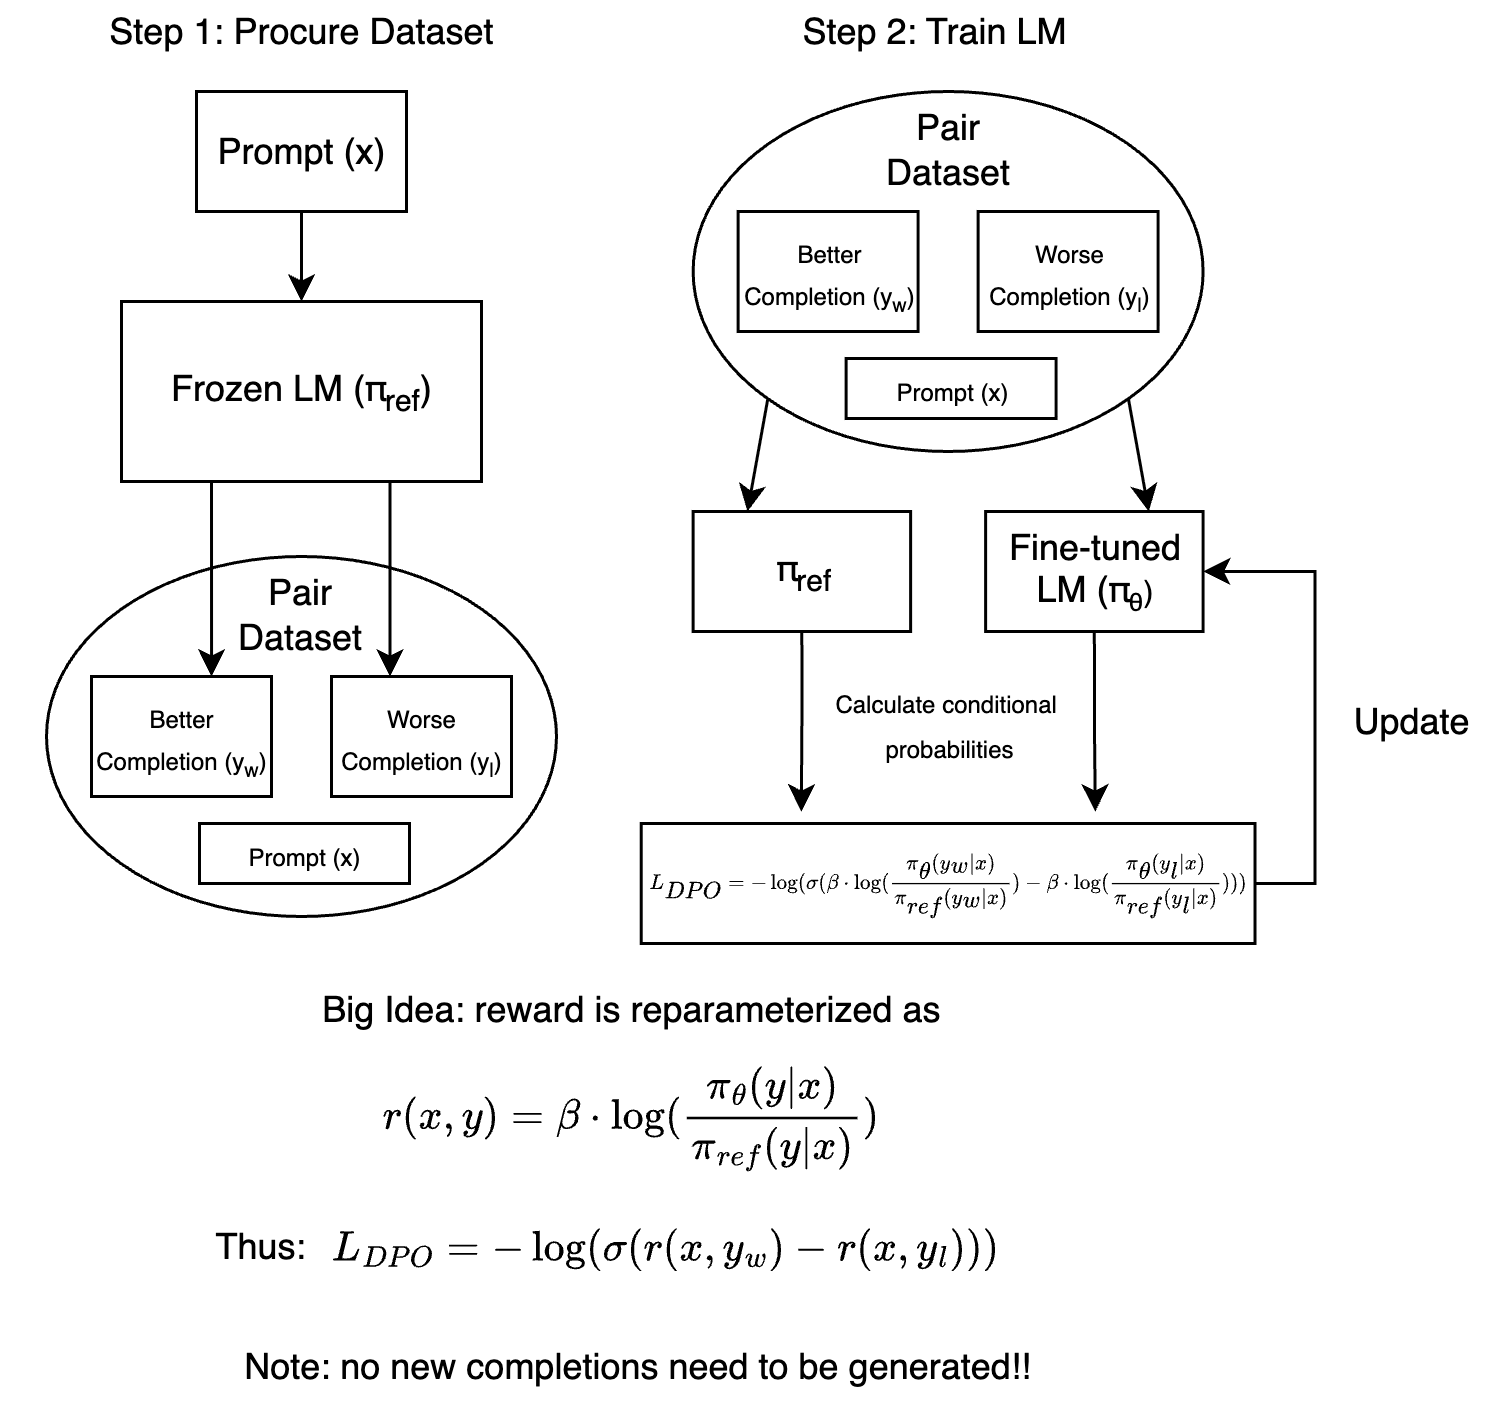
\includegraphics[width=0.8\textwidth]{../media/dpo_light.png}
    \caption{DPO overview.}
    \label{fig:dpo}
\end{figure}

DPO eliminates the need for training an explicit reward model. The loss is formatted as $L_{DPO} = \log(\sigma(r_{\theta}(x, y_w) - r_{\theta}(x, y_l)))$. The goal is to reparameterize the reward function $r_{\theta}$ such that it's in terms of the original LM outputs (thus removing the need to train a separate reward model). Specifically, $r_{\theta}(x,y)$ is reparameterized as $
\beta \log(\frac{\pi_{\theta}(y | x)}{\pi_{ref}(y | x)}) + \beta Z(x)$. Briefly, $Z(x)$ is a partition function that represents some normalization factor over all possible outputs for the LM. For more information on the mathematical justification and details, visit the paper. Because we take the difference between $r_{\theta}(x, y_w)$ and $r_{\theta}(x, y_l)$, the $Z(x)$ term cancels out, which saves us a lot of time! Thus, the final loss is represented as:
\[
L_{DPO}=-\log(\sigma(\beta \cdot \log(\frac{\pi_{\theta}(y_w | x)}{\pi_{ref}(y_w | x)}) - \beta \cdot \log(\frac{\pi_{\theta}(y_l | x)}{\pi_{ref}(y_l | x)})))
\]

The authors argue that the intuition for why this approach works so well is because LMs can natively encode reward (hence \enquote{your language model is secretly a reward model}). Notably, DPO assumes the validity of the Bradley-Terry model. This states that human preference can be modeled by scalar values and pairwise comparisons are valid methods of determining the best model output. In reality, human preference is often not transitive (i.e. preferring A over B and preferring B over C does not always guarantee A is better than C). This is also a fundamental limitation for the normal RLHF setup. 

\subsection{Resources}
\begin{itemize}
    \item \href{https://arxiv.org/pdf/2203.02155}{Training language models to follow instructions with human feedback (RLHF paper)}
    
    \item \href{https://huggingface.co/blog/deep-rl-ppo}{PPO explained more in-depth}

    \item \href{https://arxiv.org/pdf/2305.18290}{Direct Preference Optimization: Your Language Model is Secretly a Reward Model}
\end{itemize}

% \listoffigures

\end{document}